% Options for packages loaded elsewhere
\PassOptionsToPackage{unicode}{hyperref}
\PassOptionsToPackage{hyphens}{url}
%
\documentclass[
]{article}
\usepackage{amsmath,amssymb}
\usepackage{lmodern}
\usepackage{iftex}
\ifPDFTeX
  \usepackage[T1]{fontenc}
  \usepackage[utf8]{inputenc}
  \usepackage{textcomp} % provide euro and other symbols
\else % if luatex or xetex
  \usepackage{unicode-math}
  \defaultfontfeatures{Scale=MatchLowercase}
  \defaultfontfeatures[\rmfamily]{Ligatures=TeX,Scale=1}
\fi
% Use upquote if available, for straight quotes in verbatim environments
\IfFileExists{upquote.sty}{\usepackage{upquote}}{}
\IfFileExists{microtype.sty}{% use microtype if available
  \usepackage[]{microtype}
  \UseMicrotypeSet[protrusion]{basicmath} % disable protrusion for tt fonts
}{}
\makeatletter
\@ifundefined{KOMAClassName}{% if non-KOMA class
  \IfFileExists{parskip.sty}{%
    \usepackage{parskip}
  }{% else
    \setlength{\parindent}{0pt}
    \setlength{\parskip}{6pt plus 2pt minus 1pt}}
}{% if KOMA class
  \KOMAoptions{parskip=half}}
\makeatother
\usepackage{xcolor}
\usepackage[margin=1in]{geometry}
\usepackage{color}
\usepackage{fancyvrb}
\newcommand{\VerbBar}{|}
\newcommand{\VERB}{\Verb[commandchars=\\\{\}]}
\DefineVerbatimEnvironment{Highlighting}{Verbatim}{commandchars=\\\{\}}
% Add ',fontsize=\small' for more characters per line
\usepackage{framed}
\definecolor{shadecolor}{RGB}{248,248,248}
\newenvironment{Shaded}{\begin{snugshade}}{\end{snugshade}}
\newcommand{\AlertTok}[1]{\textcolor[rgb]{0.94,0.16,0.16}{#1}}
\newcommand{\AnnotationTok}[1]{\textcolor[rgb]{0.56,0.35,0.01}{\textbf{\textit{#1}}}}
\newcommand{\AttributeTok}[1]{\textcolor[rgb]{0.77,0.63,0.00}{#1}}
\newcommand{\BaseNTok}[1]{\textcolor[rgb]{0.00,0.00,0.81}{#1}}
\newcommand{\BuiltInTok}[1]{#1}
\newcommand{\CharTok}[1]{\textcolor[rgb]{0.31,0.60,0.02}{#1}}
\newcommand{\CommentTok}[1]{\textcolor[rgb]{0.56,0.35,0.01}{\textit{#1}}}
\newcommand{\CommentVarTok}[1]{\textcolor[rgb]{0.56,0.35,0.01}{\textbf{\textit{#1}}}}
\newcommand{\ConstantTok}[1]{\textcolor[rgb]{0.00,0.00,0.00}{#1}}
\newcommand{\ControlFlowTok}[1]{\textcolor[rgb]{0.13,0.29,0.53}{\textbf{#1}}}
\newcommand{\DataTypeTok}[1]{\textcolor[rgb]{0.13,0.29,0.53}{#1}}
\newcommand{\DecValTok}[1]{\textcolor[rgb]{0.00,0.00,0.81}{#1}}
\newcommand{\DocumentationTok}[1]{\textcolor[rgb]{0.56,0.35,0.01}{\textbf{\textit{#1}}}}
\newcommand{\ErrorTok}[1]{\textcolor[rgb]{0.64,0.00,0.00}{\textbf{#1}}}
\newcommand{\ExtensionTok}[1]{#1}
\newcommand{\FloatTok}[1]{\textcolor[rgb]{0.00,0.00,0.81}{#1}}
\newcommand{\FunctionTok}[1]{\textcolor[rgb]{0.00,0.00,0.00}{#1}}
\newcommand{\ImportTok}[1]{#1}
\newcommand{\InformationTok}[1]{\textcolor[rgb]{0.56,0.35,0.01}{\textbf{\textit{#1}}}}
\newcommand{\KeywordTok}[1]{\textcolor[rgb]{0.13,0.29,0.53}{\textbf{#1}}}
\newcommand{\NormalTok}[1]{#1}
\newcommand{\OperatorTok}[1]{\textcolor[rgb]{0.81,0.36,0.00}{\textbf{#1}}}
\newcommand{\OtherTok}[1]{\textcolor[rgb]{0.56,0.35,0.01}{#1}}
\newcommand{\PreprocessorTok}[1]{\textcolor[rgb]{0.56,0.35,0.01}{\textit{#1}}}
\newcommand{\RegionMarkerTok}[1]{#1}
\newcommand{\SpecialCharTok}[1]{\textcolor[rgb]{0.00,0.00,0.00}{#1}}
\newcommand{\SpecialStringTok}[1]{\textcolor[rgb]{0.31,0.60,0.02}{#1}}
\newcommand{\StringTok}[1]{\textcolor[rgb]{0.31,0.60,0.02}{#1}}
\newcommand{\VariableTok}[1]{\textcolor[rgb]{0.00,0.00,0.00}{#1}}
\newcommand{\VerbatimStringTok}[1]{\textcolor[rgb]{0.31,0.60,0.02}{#1}}
\newcommand{\WarningTok}[1]{\textcolor[rgb]{0.56,0.35,0.01}{\textbf{\textit{#1}}}}
\usepackage{graphicx}
\makeatletter
\def\maxwidth{\ifdim\Gin@nat@width>\linewidth\linewidth\else\Gin@nat@width\fi}
\def\maxheight{\ifdim\Gin@nat@height>\textheight\textheight\else\Gin@nat@height\fi}
\makeatother
% Scale images if necessary, so that they will not overflow the page
% margins by default, and it is still possible to overwrite the defaults
% using explicit options in \includegraphics[width, height, ...]{}
\setkeys{Gin}{width=\maxwidth,height=\maxheight,keepaspectratio}
% Set default figure placement to htbp
\makeatletter
\def\fps@figure{htbp}
\makeatother
\setlength{\emergencystretch}{3em} % prevent overfull lines
\providecommand{\tightlist}{%
  \setlength{\itemsep}{0pt}\setlength{\parskip}{0pt}}
\setcounter{secnumdepth}{5}
\ifLuaTeX
  \usepackage{selnolig}  % disable illegal ligatures
\fi
\IfFileExists{bookmark.sty}{\usepackage{bookmark}}{\usepackage{hyperref}}
\IfFileExists{xurl.sty}{\usepackage{xurl}}{} % add URL line breaks if available
\urlstyle{same} % disable monospaced font for URLs
\hypersetup{
  pdftitle={HUDM6122 Homework\_04},
  pdfauthor={Chenguang Pan},
  hidelinks,
  pdfcreator={LaTeX via pandoc}}

\title{HUDM6122 Homework\_04}
\author{Chenguang Pan}
\date{2023-03-01}

\begin{document}
\maketitle

\hypertarget{ex-4.1}{%
\subsection{Ex 4.1}\label{ex-4.1}}

\emph{Consider 51 objects O1, . , O51 assumed to be arranged along a
straight line with the jth object being located at a point with
coordinate j. Define the similarity sij between object i and object j
as\ldots and then apply classical multidimensional scaling to the
resulting dissimilarity matrix. Explain the shape of the derived
two-dimensional solution.}

\textbf{MY SOLUTION:}\\
First, I define the function of dissimilarities \(\delta_{ij}\) as
follows, where the input paramter \(X\) is a n*1 matrix that contains
all the coordination of 51 objects.

\begin{Shaded}
\begin{Highlighting}[]
\SpecialCharTok{\textgreater{}}\NormalTok{ D\_dis }\OtherTok{\textless{}{-}} \ControlFlowTok{function}\NormalTok{(X) \{}
\SpecialCharTok{+}\NormalTok{   n }\OtherTok{\textless{}{-}} \FunctionTok{dim}\NormalTok{(X)[}\DecValTok{1}\NormalTok{] }\CommentTok{\# to have the length of any input n*1 matrix}
\SpecialCharTok{+}\NormalTok{   S }\OtherTok{\textless{}{-}} \FunctionTok{matrix}\NormalTok{(}\DecValTok{0}\NormalTok{, n, n) }\CommentTok{\# to make a n*n empty matrix }
\SpecialCharTok{+}\NormalTok{   D }\OtherTok{\textless{}{-}} \FunctionTok{matrix}\NormalTok{(}\DecValTok{0}\NormalTok{, n, n) }\CommentTok{\# to make a n*n empty matrix }
\SpecialCharTok{+}   \CommentTok{\# to make the similarity matrix by conditions}
\SpecialCharTok{+}   \ControlFlowTok{for}\NormalTok{ (i }\ControlFlowTok{in} \FunctionTok{c}\NormalTok{(}\DecValTok{1}\SpecialCharTok{:}\NormalTok{n)) \{}
\SpecialCharTok{+}     \ControlFlowTok{for}\NormalTok{ (j }\ControlFlowTok{in} \FunctionTok{c}\NormalTok{(}\DecValTok{1}\SpecialCharTok{:}\NormalTok{n))\{}
\SpecialCharTok{+}       \ControlFlowTok{if}\NormalTok{ (i }\SpecialCharTok{==}\NormalTok{ j)\{S[i,j] }\OtherTok{\textless{}{-}} \DecValTok{9}\NormalTok{\}}
\SpecialCharTok{+}       \ControlFlowTok{else} \ControlFlowTok{if}\NormalTok{ (}\FunctionTok{abs}\NormalTok{(i}\SpecialCharTok{{-}}\NormalTok{j) }\SpecialCharTok{\textgreater{}=} \DecValTok{1} \SpecialCharTok{\&} \FunctionTok{abs}\NormalTok{(i}\SpecialCharTok{{-}}\NormalTok{j) }\SpecialCharTok{\textless{}=} \DecValTok{3}\NormalTok{)\{S[i,j] }\OtherTok{\textless{}{-}} \DecValTok{8}\NormalTok{\}}
\SpecialCharTok{+}       \ControlFlowTok{else} \ControlFlowTok{if}\NormalTok{ (}\FunctionTok{abs}\NormalTok{(i}\SpecialCharTok{{-}}\NormalTok{j) }\SpecialCharTok{\textgreater{}=} \DecValTok{4} \SpecialCharTok{\&} \FunctionTok{abs}\NormalTok{(i}\SpecialCharTok{{-}}\NormalTok{j) }\SpecialCharTok{\textless{}=} \DecValTok{6}\NormalTok{)\{S[i,j] }\OtherTok{\textless{}{-}} \DecValTok{7}\NormalTok{\}}
\SpecialCharTok{+}       \ControlFlowTok{else} \ControlFlowTok{if}\NormalTok{ (}\FunctionTok{abs}\NormalTok{(i}\SpecialCharTok{{-}}\NormalTok{j) }\SpecialCharTok{\textgreater{}=} \DecValTok{7} \SpecialCharTok{\&} \FunctionTok{abs}\NormalTok{(i}\SpecialCharTok{{-}}\NormalTok{j) }\SpecialCharTok{\textless{}=} \DecValTok{9}\NormalTok{)\{S[i,j] }\OtherTok{\textless{}{-}} \DecValTok{6}\NormalTok{\}}
\SpecialCharTok{+}       \ControlFlowTok{else} \ControlFlowTok{if}\NormalTok{ (}\FunctionTok{abs}\NormalTok{(i}\SpecialCharTok{{-}}\NormalTok{j) }\SpecialCharTok{\textgreater{}=} \DecValTok{10} \SpecialCharTok{\&} \FunctionTok{abs}\NormalTok{(i}\SpecialCharTok{{-}}\NormalTok{j) }\SpecialCharTok{\textless{}=} \DecValTok{12}\NormalTok{)\{S[i,j] }\OtherTok{\textless{}{-}} \DecValTok{5}\NormalTok{\}}
\SpecialCharTok{+}       \ControlFlowTok{else} \ControlFlowTok{if}\NormalTok{ (}\FunctionTok{abs}\NormalTok{(i}\SpecialCharTok{{-}}\NormalTok{j) }\SpecialCharTok{\textgreater{}=} \DecValTok{13} \SpecialCharTok{\&} \FunctionTok{abs}\NormalTok{(i}\SpecialCharTok{{-}}\NormalTok{j) }\SpecialCharTok{\textless{}=} \DecValTok{15}\NormalTok{)\{S[i,j] }\OtherTok{\textless{}{-}} \DecValTok{4}\NormalTok{\}}
\SpecialCharTok{+}       \ControlFlowTok{else} \ControlFlowTok{if}\NormalTok{ (}\FunctionTok{abs}\NormalTok{(i}\SpecialCharTok{{-}}\NormalTok{j) }\SpecialCharTok{\textgreater{}=} \DecValTok{16} \SpecialCharTok{\&} \FunctionTok{abs}\NormalTok{(i}\SpecialCharTok{{-}}\NormalTok{j) }\SpecialCharTok{\textless{}=} \DecValTok{18}\NormalTok{)\{S[i,j] }\OtherTok{\textless{}{-}} \DecValTok{3}\NormalTok{\}}
\SpecialCharTok{+}       \ControlFlowTok{else} \ControlFlowTok{if}\NormalTok{ (}\FunctionTok{abs}\NormalTok{(i}\SpecialCharTok{{-}}\NormalTok{j) }\SpecialCharTok{\textgreater{}=} \DecValTok{19} \SpecialCharTok{\&} \FunctionTok{abs}\NormalTok{(i}\SpecialCharTok{{-}}\NormalTok{j) }\SpecialCharTok{\textless{}=} \DecValTok{21}\NormalTok{)\{S[i,j] }\OtherTok{\textless{}{-}} \DecValTok{2}\NormalTok{\}}
\SpecialCharTok{+}       \ControlFlowTok{else} \ControlFlowTok{if}\NormalTok{ (}\FunctionTok{abs}\NormalTok{(i}\SpecialCharTok{{-}}\NormalTok{j) }\SpecialCharTok{\textgreater{}=} \DecValTok{22} \SpecialCharTok{\&} \FunctionTok{abs}\NormalTok{(i}\SpecialCharTok{{-}}\NormalTok{j) }\SpecialCharTok{\textless{}=} \DecValTok{24}\NormalTok{)\{S[i,j] }\OtherTok{\textless{}{-}} \DecValTok{1}\NormalTok{\}}
\SpecialCharTok{+}       \ControlFlowTok{else} \ControlFlowTok{if}\NormalTok{ (}\FunctionTok{abs}\NormalTok{(i}\SpecialCharTok{{-}}\NormalTok{j) }\SpecialCharTok{\textgreater{}=} \DecValTok{25}\NormalTok{)\{S[i,j] }\OtherTok{\textless{}{-}} \DecValTok{0}\NormalTok{\}}
\SpecialCharTok{+}\NormalTok{     \}}
\SpecialCharTok{+}\NormalTok{   \} }\CommentTok{\# similarity matrix finished!}
\SpecialCharTok{+}   \CommentTok{\# using the elements in the Similarity matrix to generate Dissimilarities Matrix}
\SpecialCharTok{+}   \ControlFlowTok{for}\NormalTok{ (i }\ControlFlowTok{in} \FunctionTok{c}\NormalTok{(}\DecValTok{1}\SpecialCharTok{:}\NormalTok{n)) \{}
\SpecialCharTok{+}     \ControlFlowTok{for}\NormalTok{ (j }\ControlFlowTok{in} \FunctionTok{c}\NormalTok{(}\DecValTok{1}\SpecialCharTok{:}\NormalTok{n)) \{}
\SpecialCharTok{+}\NormalTok{       D[i,j] }\OtherTok{\textless{}{-}} \FunctionTok{sqrt}\NormalTok{(S[i,i] }\SpecialCharTok{+}\NormalTok{ S[j,j] }\SpecialCharTok{{-}} \DecValTok{2}\SpecialCharTok{*}\NormalTok{S[i,j])}
\SpecialCharTok{+}\NormalTok{     \}}
\SpecialCharTok{+}\NormalTok{   \} }\CommentTok{\# dissimilarity matrix finished!}
\SpecialCharTok{+}   \FunctionTok{return}\NormalTok{(D)}
\SpecialCharTok{+}\NormalTok{ \}}
\end{Highlighting}
\end{Shaded}

Next, I randomly generate a n*1 matrix with 51 integers by using
\texttt{sample()} function. And plug this vector to the dissimilarity
function above.

\begin{Shaded}
\begin{Highlighting}[]
\SpecialCharTok{\textgreater{}}\NormalTok{ obs\_ }\OtherTok{\textless{}{-}} \ControlFlowTok{function}\NormalTok{(n) \{}
\SpecialCharTok{+}\NormalTok{   number\_vec }\OtherTok{\textless{}{-}} \FunctionTok{c}\NormalTok{(}\DecValTok{1}\SpecialCharTok{:}\NormalTok{n)}
\SpecialCharTok{+}   \CommentTok{\# change the number array to matrix}
\SpecialCharTok{+}   \FunctionTok{return}\NormalTok{(}\FunctionTok{matrix}\NormalTok{(number\_vec,n,}\DecValTok{1}\NormalTok{))}
\SpecialCharTok{+}\NormalTok{ \}}
\end{Highlighting}
\end{Shaded}

The functions above looks good. I try to generate 51 observations and
plug them into the dissimilarity matrix function to get the required D
matrix.

\begin{Shaded}
\begin{Highlighting}[]
\SpecialCharTok{\textgreater{}} \CommentTok{\# generate 51 observations}
\ErrorTok{\textgreater{}}\NormalTok{ observations }\OtherTok{\textless{}{-}} \FunctionTok{obs\_}\NormalTok{(}\DecValTok{51}\NormalTok{)}
\SpecialCharTok{\textgreater{}} \CommentTok{\# plug the n*1 matrix into the dissimilarity martix function}
\ErrorTok{\textgreater{}}\NormalTok{ D }\OtherTok{\textless{}{-}} \FunctionTok{D\_dis}\NormalTok{(observations)}
\SpecialCharTok{\textgreater{}} \CommentTok{\# select a part of the dissimilarity matrix}
\ErrorTok{\textgreater{}}\NormalTok{ D[}\DecValTok{1}\SpecialCharTok{:}\DecValTok{5}\NormalTok{,}\DecValTok{1}\SpecialCharTok{:}\DecValTok{5}\NormalTok{]}
\NormalTok{         [,}\DecValTok{1}\NormalTok{]     [,}\DecValTok{2}\NormalTok{]     [,}\DecValTok{3}\NormalTok{]     [,}\DecValTok{4}\NormalTok{]     [,}\DecValTok{5}\NormalTok{]}
\NormalTok{[}\DecValTok{1}\NormalTok{,] }\FloatTok{0.000000} \FloatTok{1.414214} \FloatTok{1.414214} \FloatTok{1.414214} \FloatTok{2.000000}
\NormalTok{[}\DecValTok{2}\NormalTok{,] }\FloatTok{1.414214} \FloatTok{0.000000} \FloatTok{1.414214} \FloatTok{1.414214} \FloatTok{1.414214}
\NormalTok{[}\DecValTok{3}\NormalTok{,] }\FloatTok{1.414214} \FloatTok{1.414214} \FloatTok{0.000000} \FloatTok{1.414214} \FloatTok{1.414214}
\NormalTok{[}\DecValTok{4}\NormalTok{,] }\FloatTok{1.414214} \FloatTok{1.414214} \FloatTok{1.414214} \FloatTok{0.000000} \FloatTok{1.414214}
\NormalTok{[}\DecValTok{5}\NormalTok{,] }\FloatTok{2.000000} \FloatTok{1.414214} \FloatTok{1.414214} \FloatTok{1.414214} \FloatTok{0.000000}
\end{Highlighting}
\end{Shaded}

This dissimilarity matrix looks good. Then I run the classical
multidimensional scaling to this resulting matrix. Note, this is a
non-Euclidean case. Some of the eigenvalue may be negative.

\begin{Shaded}
\begin{Highlighting}[]
\SpecialCharTok{\textgreater{}}\NormalTok{ d\_mds }\OtherTok{\textless{}{-}} \FunctionTok{cmdscale}\NormalTok{(D, }\AttributeTok{k=}\DecValTok{50}\NormalTok{, }\AttributeTok{eig =}\NormalTok{ T)}
\SpecialCharTok{\textgreater{}}\NormalTok{ lam }\OtherTok{\textless{}{-}}\NormalTok{ d\_mds}\SpecialCharTok{$}\NormalTok{eig}
\SpecialCharTok{\textgreater{}} \CommentTok{\# d\_mds$points}
\ErrorTok{\textgreater{}} \FunctionTok{cumsum}\NormalTok{(}\FunctionTok{abs}\NormalTok{(lam))}\SpecialCharTok{/}\FunctionTok{sum}\NormalTok{(}\FunctionTok{abs}\NormalTok{(lam))}
\NormalTok{ [}\DecValTok{1}\NormalTok{] }\FloatTok{0.4428488} \FloatTok{0.6744323} \FloatTok{0.7382541} \FloatTok{0.7657231} \FloatTok{0.7924526} \FloatTok{0.8183668} \FloatTok{0.8430174}
\NormalTok{ [}\DecValTok{8}\NormalTok{] }\FloatTok{0.8615740} \FloatTok{0.8736449} \FloatTok{0.8845189} \FloatTok{0.8953701} \FloatTok{0.9048445} \FloatTok{0.9116561} \FloatTok{0.9167756}
\NormalTok{[}\DecValTok{15}\NormalTok{] }\FloatTok{0.9217895} \FloatTok{0.9267112} \FloatTok{0.9314246} \FloatTok{0.9355091} \FloatTok{0.9389073} \FloatTok{0.9422424} \FloatTok{0.9455372}
\NormalTok{[}\DecValTok{22}\NormalTok{] }\FloatTok{0.9486160} \FloatTok{0.9513996} \FloatTok{0.9540916} \FloatTok{0.9565647} \FloatTok{0.9589956} \FloatTok{0.9611009} \FloatTok{0.9630147}
\NormalTok{[}\DecValTok{29}\NormalTok{] }\FloatTok{0.9646832} \FloatTok{0.9663473} \FloatTok{0.9677584} \FloatTok{0.9691622} \FloatTok{0.9704291} \FloatTok{0.9714991} \FloatTok{0.9725150}
\NormalTok{[}\DecValTok{36}\NormalTok{] }\FloatTok{0.9734831} \FloatTok{0.9744191} \FloatTok{0.9753283} \FloatTok{0.9762204} \FloatTok{0.9771018} \FloatTok{0.9775266} \FloatTok{0.9778771}
\NormalTok{[}\DecValTok{43}\NormalTok{] }\FloatTok{0.9778771} \FloatTok{0.9782091} \FloatTok{0.9785814} \FloatTok{0.9796588} \FloatTok{0.9808172} \FloatTok{0.9831840} \FloatTok{0.9856796}
\NormalTok{[}\DecValTok{50}\NormalTok{] }\FloatTok{0.9927144} \FloatTok{1.0000000}
\SpecialCharTok{\textgreater{}} \FunctionTok{cumsum}\NormalTok{(}\FunctionTok{abs}\NormalTok{(lam}\SpecialCharTok{\^{}}\DecValTok{2}\NormalTok{))}\SpecialCharTok{/}\FunctionTok{sum}\NormalTok{(}\FunctionTok{abs}\NormalTok{(lam}\SpecialCharTok{\^{}}\DecValTok{2}\NormalTok{))}
\NormalTok{ [}\DecValTok{1}\NormalTok{] }\FloatTok{0.7608520} \FloatTok{0.9689196} \FloatTok{0.9847222} \FloatTok{0.9876495} \FloatTok{0.9904214} \FloatTok{0.9930267} \FloatTok{0.9953842}
\NormalTok{ [}\DecValTok{8}\NormalTok{] }\FloatTok{0.9967201} \FloatTok{0.9972854} \FloatTok{0.9977441} \FloatTok{0.9982010} \FloatTok{0.9985492} \FloatTok{0.9987292} \FloatTok{0.9988309}
\NormalTok{[}\DecValTok{15}\NormalTok{] }\FloatTok{0.9989284} \FloatTok{0.9990224} \FloatTok{0.9991086} \FloatTok{0.9991733} \FloatTok{0.9992181} \FloatTok{0.9992613} \FloatTok{0.9993034}
\NormalTok{[}\DecValTok{22}\NormalTok{] }\FloatTok{0.9993402} \FloatTok{0.9993702} \FloatTok{0.9993983} \FloatTok{0.9994221} \FloatTok{0.9994450} \FloatTok{0.9994622} \FloatTok{0.9994764}
\NormalTok{[}\DecValTok{29}\NormalTok{] }\FloatTok{0.9994872} \FloatTok{0.9994979} \FloatTok{0.9995057} \FloatTok{0.9995133} \FloatTok{0.9995195} \FloatTok{0.9995240} \FloatTok{0.9995280}
\NormalTok{[}\DecValTok{36}\NormalTok{] }\FloatTok{0.9995316} \FloatTok{0.9995350} \FloatTok{0.9995382} \FloatTok{0.9995413} \FloatTok{0.9995443} \FloatTok{0.9995450} \FloatTok{0.9995455}
\NormalTok{[}\DecValTok{43}\NormalTok{] }\FloatTok{0.9995455} \FloatTok{0.9995459} \FloatTok{0.9995465} \FloatTok{0.9995510} \FloatTok{0.9995562} \FloatTok{0.9995779} \FloatTok{0.9996021}
\NormalTok{[}\DecValTok{50}\NormalTok{] }\FloatTok{0.9997941} \FloatTok{1.0000000}
\end{Highlighting}
\end{Shaded}

These values suggest that the first two coordinates will give an
adequate representation of the simulated dissimilarity distances. Then,
I make the scatter plot using the first two scores.

\begin{Shaded}
\begin{Highlighting}[]
\SpecialCharTok{\textgreater{}}\NormalTok{ lim }\OtherTok{\textless{}{-}} \FunctionTok{range}\NormalTok{(d\_mds}\SpecialCharTok{$}\NormalTok{points[,}\DecValTok{1}\NormalTok{] }\SpecialCharTok{*}\NormalTok{ (}\SpecialCharTok{{-}}\DecValTok{1}\NormalTok{)) }\SpecialCharTok{*} \FloatTok{1.2}
\SpecialCharTok{\textgreater{}} 
\ErrorTok{\textgreater{}} \FunctionTok{plot}\NormalTok{(d\_mds}\SpecialCharTok{$}\NormalTok{points[,}\DecValTok{1}\NormalTok{]}\SpecialCharTok{*}\NormalTok{(}\SpecialCharTok{{-}}\DecValTok{1}\NormalTok{), d\_mds}\SpecialCharTok{$}\NormalTok{points[,}\DecValTok{2}\NormalTok{]}\SpecialCharTok{*}\NormalTok{(}\SpecialCharTok{{-}}\DecValTok{1}\NormalTok{), }
\SpecialCharTok{+}      \AttributeTok{xlab =} \StringTok{"Coordinate 1"}\NormalTok{, }\AttributeTok{ylab =} \StringTok{"Coordinate 2"}\NormalTok{,}
\SpecialCharTok{+}      \AttributeTok{xlim =}\NormalTok{ lim, }\AttributeTok{ylim =}\NormalTok{ lim)}
\end{Highlighting}
\end{Shaded}

\begin{Shaded}
\begin{Highlighting}[]
\SpecialCharTok{\textgreater{}}\NormalTok{ lim }\OtherTok{\textless{}{-}} \FunctionTok{range}\NormalTok{(d\_mds}\SpecialCharTok{$}\NormalTok{points[,}\DecValTok{1}\NormalTok{]) }\SpecialCharTok{*} \FloatTok{1.2}
\SpecialCharTok{\textgreater{}} \FunctionTok{plot}\NormalTok{(d\_mds}\SpecialCharTok{$}\NormalTok{points[,}\DecValTok{1}\NormalTok{], d\_mds}\SpecialCharTok{$}\NormalTok{points[,}\DecValTok{2}\NormalTok{], }
\SpecialCharTok{+}      \AttributeTok{xlab =} \StringTok{"Coordinate 1"}\NormalTok{, }\AttributeTok{ylab =} \StringTok{"Coordinate 2"}\NormalTok{,}
\SpecialCharTok{+}      \AttributeTok{xlim =}\NormalTok{ lim, }\AttributeTok{ylim =}\NormalTok{ lim)}
\SpecialCharTok{\textgreater{}} \FunctionTok{text}\NormalTok{(d\_mds}\SpecialCharTok{$}\NormalTok{points[,}\DecValTok{1}\NormalTok{], d\_mds}\SpecialCharTok{$}\NormalTok{points[,}\DecValTok{2}\NormalTok{], }\AttributeTok{labels =} \FunctionTok{c}\NormalTok{(}\DecValTok{1}\SpecialCharTok{:}\DecValTok{51}\NormalTok{), }\AttributeTok{pos=}\DecValTok{2}\NormalTok{,}\AttributeTok{cex =} \FloatTok{0.7}\NormalTok{)}
\end{Highlighting}
\end{Shaded}

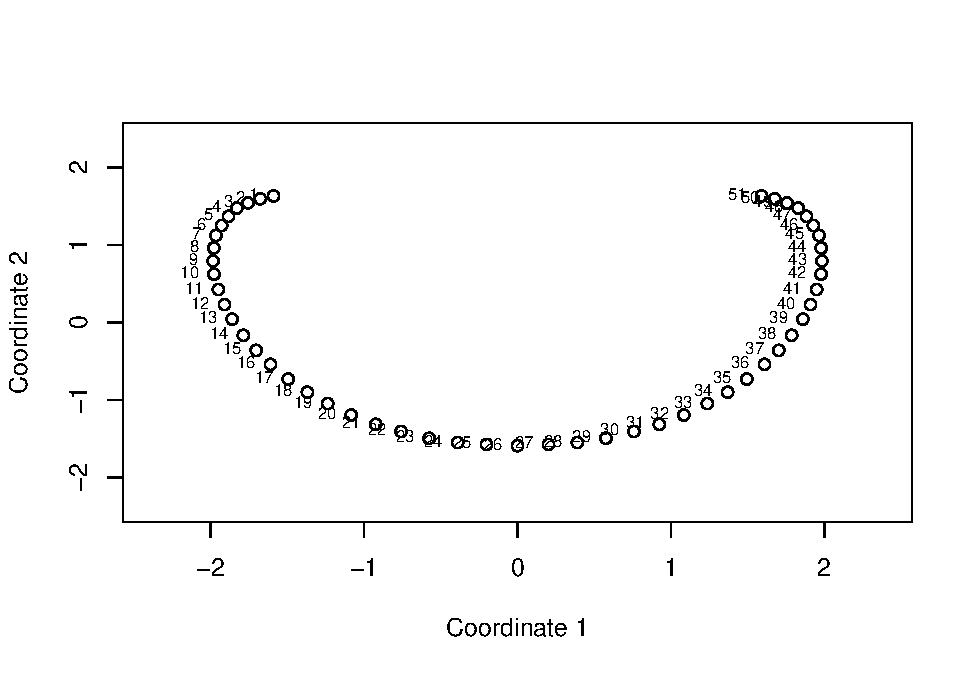
\includegraphics{HUDM6122-Homework_04-Chenguang-Pan_files/figure-latex/unnamed-chunk-7-1.pdf}
This two-dimensional plot has the symmetrical shape, which is reasonable
since the mid-point,i.e., the 26th point, has the same dissimilarity
with both the points on its left and right. Therefore, if we project all
point on y-axis, it actually represent the dissimilarity degree between
the each point and the 26th point.

\hypertarget{ex.-4.2}{%
\subsection{Ex. 4.2}\label{ex.-4.2}}

\emph{Write an R function to calculate the chi-squared distance matrices
for both rows and columns in a two-dimensional contingency table.}

\textbf{MY SOLUTION} Based on the definition of chi-squared distance
matrices, I write the function as follows:

\begin{Shaded}
\begin{Highlighting}[]
\SpecialCharTok{\textgreater{}}\NormalTok{ chi\_squared\_dist\_matrices }\OtherTok{\textless{}{-}} \ControlFlowTok{function}\NormalTok{(tbl)\{}
\SpecialCharTok{+}   \CommentTok{\# Calculate row sums and column sums}
\SpecialCharTok{+}\NormalTok{   row\_sums }\OtherTok{\textless{}{-}} \FunctionTok{apply}\NormalTok{(tbl, }\DecValTok{1}\NormalTok{, sum)}
\SpecialCharTok{+}\NormalTok{   col\_sums }\OtherTok{\textless{}{-}} \FunctionTok{apply}\NormalTok{(tbl, }\DecValTok{2}\NormalTok{, sum)}
\SpecialCharTok{+}   \CommentTok{\# Calculate total count and expected counts}
\SpecialCharTok{+}\NormalTok{   total\_count }\OtherTok{\textless{}{-}} \FunctionTok{sum}\NormalTok{(tbl)}
\SpecialCharTok{+}   
\SpecialCharTok{+}   \CommentTok{\# to have the dim of the input matrix}
\SpecialCharTok{+}\NormalTok{   c }\OtherTok{\textless{}{-}} \FunctionTok{ncol}\NormalTok{(tbl)}
\SpecialCharTok{+}\NormalTok{   r }\OtherTok{\textless{}{-}} \FunctionTok{nrow}\NormalTok{(tbl)}
\SpecialCharTok{+}   \CommentTok{\# make a empty matrix to load all elements}
\SpecialCharTok{+}\NormalTok{   col\_d\_matrix }\OtherTok{\textless{}{-}} \FunctionTok{matrix}\NormalTok{(}\DecValTok{0}\NormalTok{,c,c)}
\SpecialCharTok{+}   
\SpecialCharTok{+}   \CommentTok{\# using loop to write the each ij entries into this matrix}
\SpecialCharTok{+}   \ControlFlowTok{for}\NormalTok{ (i }\ControlFlowTok{in} \FunctionTok{c}\NormalTok{(}\DecValTok{1}\SpecialCharTok{:}\NormalTok{c)) \{}
\SpecialCharTok{+}     \ControlFlowTok{for}\NormalTok{ (j }\ControlFlowTok{in} \FunctionTok{c}\NormalTok{(}\DecValTok{1}\SpecialCharTok{:}\NormalTok{c)) \{}
\SpecialCharTok{+}\NormalTok{       d\_ij }\OtherTok{\textless{}{-}} \DecValTok{0}
\SpecialCharTok{+}       \ControlFlowTok{for}\NormalTok{ (k }\ControlFlowTok{in} \FunctionTok{c}\NormalTok{(}\DecValTok{1}\SpecialCharTok{:}\NormalTok{r)) \{}
\SpecialCharTok{+}\NormalTok{         p\_k\_dot }\OtherTok{\textless{}{-}}\NormalTok{ row\_sums[k]}\SpecialCharTok{/}\NormalTok{total\_count}
\SpecialCharTok{+}\NormalTok{         p\_k\_i }\OtherTok{\textless{}{-}}\NormalTok{ tbl[k,i]}\SpecialCharTok{/}\NormalTok{col\_sums[i]}
\SpecialCharTok{+}\NormalTok{         p\_k\_j }\OtherTok{\textless{}{-}}\NormalTok{ tbl[k,j]}\SpecialCharTok{/}\NormalTok{col\_sums[j]}
\SpecialCharTok{+}\NormalTok{         d\_ij }\OtherTok{\textless{}{-}}\NormalTok{ d\_ij }\SpecialCharTok{+}\NormalTok{ (}\DecValTok{1}\SpecialCharTok{/}\NormalTok{p\_k\_dot)}\SpecialCharTok{*}\NormalTok{(p\_k\_i}\SpecialCharTok{{-}}\NormalTok{p\_k\_j)}\SpecialCharTok{\^{}}\DecValTok{2}
\SpecialCharTok{+}\NormalTok{       \}}
\SpecialCharTok{+}\NormalTok{       col\_d\_matrix[i,j] }\OtherTok{\textless{}{-}}\NormalTok{ d\_ij}
\SpecialCharTok{+}\NormalTok{     \}}
\SpecialCharTok{+}\NormalTok{   \}}
\SpecialCharTok{+}   \CommentTok{\# make a empty matrix to load all elements}
\SpecialCharTok{+}\NormalTok{   row\_d\_matrix }\OtherTok{\textless{}{-}} \FunctionTok{matrix}\NormalTok{(}\DecValTok{0}\NormalTok{,r,r)}
\SpecialCharTok{+}   
\SpecialCharTok{+}   \CommentTok{\# using loop to write the each ij entries into this matrix}
\SpecialCharTok{+}   \ControlFlowTok{for}\NormalTok{ (i }\ControlFlowTok{in} \FunctionTok{c}\NormalTok{(}\DecValTok{1}\SpecialCharTok{:}\NormalTok{r)) \{}
\SpecialCharTok{+}     \ControlFlowTok{for}\NormalTok{ (j }\ControlFlowTok{in} \FunctionTok{c}\NormalTok{(}\DecValTok{1}\SpecialCharTok{:}\NormalTok{r)) \{}
\SpecialCharTok{+}\NormalTok{       d\_ij }\OtherTok{\textless{}{-}} \DecValTok{0}
\SpecialCharTok{+}       \ControlFlowTok{for}\NormalTok{ (k }\ControlFlowTok{in} \FunctionTok{c}\NormalTok{(}\DecValTok{1}\SpecialCharTok{:}\NormalTok{r)) \{}
\SpecialCharTok{+}\NormalTok{         p\_dot\_k }\OtherTok{\textless{}{-}}\NormalTok{ col\_sums[k]}\SpecialCharTok{/}\NormalTok{total\_count}
\SpecialCharTok{+}\NormalTok{         p\_i\_k }\OtherTok{\textless{}{-}}\NormalTok{ tbl[i,k]}\SpecialCharTok{/}\NormalTok{row\_sums[i]}
\SpecialCharTok{+}\NormalTok{         p\_j\_k }\OtherTok{\textless{}{-}}\NormalTok{ tbl[j,k]}\SpecialCharTok{/}\NormalTok{row\_sums[j]}
\SpecialCharTok{+}\NormalTok{         d\_ij }\OtherTok{\textless{}{-}}\NormalTok{ d\_ij }\SpecialCharTok{+}\NormalTok{ (}\DecValTok{1}\SpecialCharTok{/}\NormalTok{p\_dot\_k)}\SpecialCharTok{*}\NormalTok{(p\_i\_k}\SpecialCharTok{{-}}\NormalTok{p\_j\_k)}\SpecialCharTok{\^{}}\DecValTok{2}
\SpecialCharTok{+}\NormalTok{       \}}
\SpecialCharTok{+}\NormalTok{       row\_d\_matrix[i,j] }\OtherTok{\textless{}{-}}\NormalTok{ d\_ij}
\SpecialCharTok{+}\NormalTok{     \}}
\SpecialCharTok{+}\NormalTok{   \}}
\SpecialCharTok{+}   \FunctionTok{return}\NormalTok{(}\FunctionTok{list}\NormalTok{(col\_d\_matrix, row\_d\_matrix))}
\SpecialCharTok{+}\NormalTok{ \}}
\end{Highlighting}
\end{Shaded}

This function return a list that contains both columns distance matrix
and rows distance matrix. By using the index, like
\texttt{{[}{[}1{]}{]}}or \texttt{{[}{[}2{]}{]}}, to extract the columns
or rows distance matrix, respectively. Next, I created a two-dimensional
contigency table to test this function.

\begin{Shaded}
\begin{Highlighting}[]
\SpecialCharTok{\textgreater{}} \CommentTok{\# Create a contingency table}
\ErrorTok{\textgreater{}}\NormalTok{ tbl }\OtherTok{\textless{}{-}} \FunctionTok{table}\NormalTok{(}\FunctionTok{c}\NormalTok{(}\StringTok{"A"}\NormalTok{, }\StringTok{"A"}\NormalTok{, }\StringTok{"B"}\NormalTok{, }\StringTok{"B"}\NormalTok{), }\FunctionTok{c}\NormalTok{(}\StringTok{"X"}\NormalTok{, }\StringTok{"Y"}\NormalTok{, }\StringTok{"X"}\NormalTok{, }\StringTok{"Z"}\NormalTok{))}
\SpecialCharTok{\textgreater{}}\NormalTok{ tbl}
   
\NormalTok{    X Y Z}
\NormalTok{  A }\DecValTok{1} \DecValTok{1} \DecValTok{0}
\NormalTok{  B }\DecValTok{1} \DecValTok{0} \DecValTok{1}
\SpecialCharTok{\textgreater{}} \CommentTok{\# plug this simulated table into the function above}
\ErrorTok{\textgreater{}}\NormalTok{ dist\_m }\OtherTok{\textless{}{-}}\FunctionTok{chi\_squared\_dist\_matrices}\NormalTok{(tbl)}
\SpecialCharTok{\textgreater{}} \CommentTok{\# the columns distance matrix is}
\ErrorTok{\textgreater{}}\NormalTok{ dist\_m[[}\DecValTok{1}\NormalTok{]]}
\NormalTok{     [,}\DecValTok{1}\NormalTok{] [,}\DecValTok{2}\NormalTok{] [,}\DecValTok{3}\NormalTok{]}
\NormalTok{[}\DecValTok{1}\NormalTok{,]    }\DecValTok{0}    \DecValTok{1}    \DecValTok{1}
\NormalTok{[}\DecValTok{2}\NormalTok{,]    }\DecValTok{1}    \DecValTok{0}    \DecValTok{4}
\NormalTok{[}\DecValTok{3}\NormalTok{,]    }\DecValTok{1}    \DecValTok{4}    \DecValTok{0}
\SpecialCharTok{\textgreater{}} \CommentTok{\# the row distance matrix is}
\ErrorTok{\textgreater{}}\NormalTok{ dist\_m[[}\DecValTok{2}\NormalTok{]]}
\NormalTok{     [,}\DecValTok{1}\NormalTok{] [,}\DecValTok{2}\NormalTok{]}
\NormalTok{[}\DecValTok{1}\NormalTok{,]    }\DecValTok{0}    \DecValTok{1}
\NormalTok{[}\DecValTok{2}\NormalTok{,]    }\DecValTok{1}    \DecValTok{0}
\end{Highlighting}
\end{Shaded}


\end{document}
